\chapter{(Linear) Group Actions}


If $G$ is a group then we denote by $e \in G$ the neutral element and by $gh$ the composition of $g,h \in G$ and by $g^{-1}$ the inverse of $g \in G$.


\begin{defi}
 Given a group $G$ and a set $X$ then an action of $G$ on $X$ is a map
 \[
  \pi : G \times X \to X, (g,x) \to g.x,
 \]
 such that
 \begin{gather*}
  e.x = x \text{ and }
  (gh).x = g.(h.x)
 \end{gather*}
 for all $x \in X, g,h \in G$. We say then that $X$ is a $G$-set.
\end{defi}


\begin{defi}
 Given a set $X$ let
 \[
  S(X) := \{f : X \to X | f \text{ is bijective}\}.
 \]
 $S(X)$ is then a group with $fg := f \circ g$ (composition of maps) for all $f,g \in S(X)$ and $e = \id_X$.
\end{defi}


Given a group action $\pi : G \times X \to X$ any  $g \in G$ defines $\pi_g \in S(X)$ by setting
\[
 \pi_g(x) = \pi(g.x) \text{ for all } x \in X, g \in G.
\]


\begin{lem}
 Fix $G$ a group, $X$ a set. Then there is a 1:1-correspondence
 \[
 \begin{matrix}
    \left\{\text{$G$-actions on $X$}\right\}
  & \overset{1:1}{\longleftrightarrow}
  & \left\{\text{group homomorphisms $G \to S(X)$}\right\} \\
    \pi
  & \longmapsto
  & \hat{\pi} \\
    \mathring{\varphi}
  & \longmapsfrom
  & \varphi
  \end{matrix}
 \]
 where
 \[
  \hat{\pi}(g)(x) = g.x \text{ and } \mathring{\varphi}((g,x)) = \varphi(g)(x)
 \]
 for all $x \in X, g \in G$.
\end{lem}


From this Lemma we get the idea that group actions are ``the same'' as ``representing'' groups as permutation groups.


\begin{expls}
 Let $G$ be a group.
 \begin{enumerate}
  \item
   $G$ acts on itself by left multiplication, i.e.
   \[
    g.x = gx \text{ for all } g \in G, x \in X=G.
   \]
   This is called the \emph{(left) regular action of $G$}.
  \item
   $G$ acts onto itself by right multiplication with the inverse, i.e
   \[
    g.x = xg^{-1} \text{ for all } g \in G, x \in X=G.
   \]
   This is called the \emph{right regular action}.
  \item
   $G$ acts onto itself by conjugation, i.e.
   \[
    g.x = gxg^{-1} \text{ for all }g \in G, x \in X=G.
   \]
  \item
   Let $X$ be any set. Then $g.x = x$ for all $g \in G, x \in X$ defines an action. This is called the \emph{trivial action} and $X$ is called a \emph{trivial $G$-set}.
  \item
   Let $X, Y$ be $G$-sets. Then
   \[
    \Maps(X,Y) = \{f | f : X \to Y\}
   \]
   is a $G$-set by setting
   \[
    (g.f)(x) = g.\left(f\left(g^{-1}.x\right)\right)
   \]
   for all $g \in G, x \in X$.
   In the special case that $Y$ is a trivial $G$-set this means $(g.f)(x) = f(g^{-1}.x)$ for all $g \in G, x \in X$.
  \item
   If $X, Y$ are $G$-sets then $X \times Y$ is a $G$-set via
   \[
    g.(x,y) = (g.x,g.y) \text{ for all } g \in G, x \in X, y \in Y.
   \]
  \item
   If $X$ is a set and $G = S(X)$, then $X$ is a $G$-set via $f.x = f(x)$ for all $f \in G, x \in X$.
 \end{enumerate}
\end{expls}


\begin{defi}
 Let $G$ be a group and $X, Y$ $G$-sets. Then $f : X \to Y$ is called G-equivalent if
 \[
  f(g.x) = g.f(x)
 \]
 for all $g \in G, x \in X$. Denote
 \[
  \Hom_G(X,Y) = \{f : X \to Y | f \text{ is $G$-equivalent}\}.
 \]
\end{defi}


\begin{lem}
 Let $G$ be a group.
 \begin{enumerate}
  \item If $X$ is a $G$-set, then $\id_X \in \Hom_G(X,X)$.
  \item If $X, Y, Z$ are $G$-sets with $f_1 \in \Hom_G(X,Y)$ and $f_2 \in \Hom_G(Y,Z)$ then $f_2 \circ f_1 \in \Hom_G(X,Z)$.
 \end{enumerate}
\end{lem}


\begin{expls}
 \begin{enumerate}
  \item
   Let $G$ be a group and look at $G$ as a regular $G$-set. Then $f : G \to G$ is $G$-equivalent if and only if $f$ is given by right multiplication with some element $a \in G$ (i.e $f(g) = ga$ for all $g \in G$).
   \begin{proof}
    Assume there exists $a \in G$ such that $f(g) = ga$ for all $g \in G$. Then
    \[
     f(g.x) = f(gx) = (gx)a = g(xa) = g.f(x)
    \]
    for all $g, x \in G$. To show the other direction set $a := f(e)$. Because $f$ is $G$-equivalent we then have
    \[
     f(g) = f(ge) = f(g.e) = g.f(e) = g.a = ga
    \]
    for all $g \in G$.
   \end{proof}
  \item
   If $X$ and $Y$ are trivial $G$-sets then $\Hom_G(X,Y) = \Maps(X,Y)$.
  \item
   If $X$ is a $G$-set and $Y$ is a trivial $G$-set then
   \[
    \Hom_G(X,Y) = \{f : X \to Y | f(g.x) = f(x) \text{ for all } g \in G, x \in X\}.
   \]
 \end{enumerate}
\end{expls}


\begin{defi}
 Let $X$ be a $G$-set. We write
 \[
  X/G := \{\text{orbits of $G$ in $X$}\}.
 \]
\end{defi}


\begin{note}
 There is an induced, but trivial action of $G$ on $X/G$ from the action of $G$ on $X$, and the canonical map
 \[
  \can : X \to X/G, x \mapsto \text{orbit of } x
 \]
 is $G$-equivalent, since
 \[
  \can(g.x) = \text{orbit of $g.x$} = \text{orbit of $x$} = \can(x) = g.\can(x)
 \]
 for all $g \in G, x \in X$.
\end{note}


\begin{defi}
 Let $X$ be a $G$-set. Then
 \[
  X^G := \{\text{$G$-invariants of $X$}\} = \{x \in X : g.x = x \text{ for all } g \in G\}.
 \]
 The elements in $X^G$ are called $G$-invariants or $G$ fix points.
\end{defi}


\begin{lem}
 Let $X, Y$ be $G$-sets. Then $\Hom_G(X,Y) = \Maps(X,Y)^G$.
\end{lem}
\begin{proof}
 \begin{align*}
  f \in \Hom_G(X,Y)
  &\Leftrightarrow \forall g \in G, x \in X : f(g.x) = g.f(x) \\
  &\Leftrightarrow \forall g \in G, x \in X : f(g^{-1}.x) = g^{-1}.f(x) \\
  &\Leftrightarrow \forall g \in G, x \in X : g.f(g^{-1}.x) = f(x) \\
  &\Leftrightarrow \forall g \in G : g.f = f \\
  &\Leftrightarrow f \in \Maps(X,Y)^G.
 \end{align*}
\end{proof}


\begin{defi}
 Let $X$ be a $G$-set, $k$ a field or a ring. $f : X \to k$ is called invariant (or better $G$-invariant) if
 \[
  f(x) = f(g^{-1}.x) \text{ for all } g \in G, x \in X.
 \]
\end{defi}


\begin{note}
 This agrees with the above definition of $f \in \Hom_G(X,k) = \Maps(X,k)^G$ if we consider $k$ as a trivial $G$-set.
\end{note}


\begin{lem}
 Let $X$ be a $G$-set, $k$ a field or a ring. Then $f : X \to k$ is invariant if and only if $f$ factors through $\can$, i.e. if the following diagram commutes.
 \begin{center}
 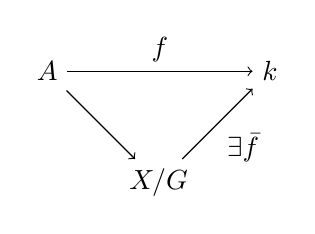
\begin{tikzpicture}[node distance = 2cm, auto]
  \node (A) {$A$};
  \node (XG) [below right of = A] {$X/G$};
  \node (k) [above right of = XG] {$k$};
  \draw[->] (A) to node {$f$} (k);
  \draw[->] (A) to node [swap] {$\can$} (XG);
  \draw[->] (XG) to node [swap] {$\exists\bar{f}$} (k);
 \end{tikzpicture}
 \end{center}
\end{lem}
\begin{proof}
 If $f$ is invariant then $f(x) = f(g^{-1}.x)$ for all $g \in G, x \in X$. Therefore $f$ is constant on orbits. Now define $\bar{f}(\mc{O}) = f(x)$ where $\mc{O}$ is an orbit and $x \in \mc{O}$.
 
 To show the other direction assume $f$ factors through $\can$. Then $f$ is constant on orbits, i.e. $f(x) = f(g.x)$ for all $g \in G, x \in X$, i.e. $f(x) = f(g^{-1}.x)$ for all $g \in G, x \in X$. Therefore $f$ is invariant.
\end{proof}


\begin{expl}
 Let $G = \Z/2 = \{e,s\}$ where $e$ is the neutral element and $s^2 = e$. Let $G$ act on $X = \R$ by $e.\lambda = \lambda$ and $s.\lambda = -\lambda$ for all $\lambda \in \R$. Set $k = \R$ and consider $\Maps(X,k) = \Maps(\R,\R)$. Any polynomial $p \in \R[X]$ can be viewed as an element in $\Maps(\R,\R)$. Take for example $p_n(X) = X^n$. We can ask ourselves which of the $p_n$’s is $G$-invariant. We need to check for which $n$ we have
 \[
  p_n(x) = p_n(s^{-1}.x) = p_n(s.x) = p_n(-x) \text{ for all } x \in \R.
 \]
 Since $p_n(X) = X^n$ we get that $p_n$ is $G$-invariant if and only if $n$ is even.
\end{expl}


\begin{lem}\label{lem: basis of Maps and Hom}
 Let $X$ be a finite $G$-set. Let $k$ be a field (or a ring).
 \begin{enumerate}[a)]
  \item
   $\Maps(X,k)$ forms a $k$-vector space (resp. $k$-module) via pointwise addition and scalar multiplication.
  \item
   A $k$-basis of $\Maps(X,k)$ is given by $\{\chi_x : x \in X\}$ where
   \[
    \chi_x(y) =
    \begin{cases}
     1 & \text{if } x=y, \\
     0 & \text{otherwise}
    \end{cases}
   \]
   for all $y \in X$.
  \item
   $\Maps(X,k)^G = \Hom_G(X,k)$ forms a $k$-vector subspace (resp. $k$-submodule) of $\Maps(X,k)$.
  \item
   A $k$-Basis of $\Maps(X,k)^G$ is given by $\{\chi_\mc{O} | \mc{O} \in X/G\}$ with
   \[
    \chi_\mc{O}(y) =
    \begin{cases}
     1 & \text{if } y \in \mc{O}, \\
     0 & \text{otherwise}
    \end{cases}
   \]
   for all $y \in X$.
 \end{enumerate}
\end{lem}
\begin{proof}
 \begin{enumerate}[a)]
  \item
   This is left as an easy exercise for the reader.
  \item
   For $f \in \Maps(X,k)$ we have $f = \sum_{x \in X} f(x) \chi_x$. (Note that this sum is finite, hence defined.) This is true because for all $y \in X$ we have
   \[
    \sum_{x \in X} f(x) \chi_x(y) = f(y).
   \]
   This shows that the $\chi_x$'s generate $\Maps(X,k)$. They are linear independent since for $\alpha_x \in K, x \in X$ with $\sum_{x \in X} \alpha_x \chi_x = 0$ we have
   \[
    \alpha_y = \sum_{x \in X} \alpha_x \chi_x(y) = 0
   \]
   for all $y \in X$.
  \item
   We need to check that for all $f_1, f_2 \in \Maps(X,k)^G$ we have $f_1+f_2 \in \Maps(X,k)^G$ and that for all $f \in \Maps(X,k)^G$ and $\lambda \in k$ we have $\lambda f \in \Maps(X,k)^G$. This holds because
   \begin{align*}
    (g.(f_1+f_2))(x)
    &= (f_1+f_2)(g^{-1}.x) = f_1(g^{-1}.x) + f_2(g^{-1}.x) \\
    &= f_1(x) + f_2(x) = (f_1+f_2)(x) \text{ and} \\
    (g.(\lambda f))(x)
    &= (\lambda f)(g^{-1}.x) = \lambda (f(g^{-1}.x)) = \lambda f(x) = (\lambda f)(x)
   \end{align*}
   for all $x \in X, \lambda \in K$.
  \item
   Let $f \in \Maps(X,k)^G$ and $\mc{O}_1, \ldots, \mc{O}_n$ be the orbits in $X$. Pick a representative $x_i \in \mc{O}_i$ for all $1 \leq i \leq n$. Then $f = \sum_{i=1}^n f(x_i) \chi_{\mc{O}_i}$. This adds because
   \[
    \sum_{i=1}^n f(x_i) \chi_{\mc{O}_i}(y) = f(x_j)
   \]
   for $j$ chosen such that $y \in \mc{O}_j$, i.e. $y = g^{-1}.x_j$ for some $g \in G$. We then have $f(y) = f(g^{-1}.x_j) = f(x_j)$. This shows that the $\chi_{\mc{O}_i}$’s generate $\Maps(X,k)^G$. The linear independence is clear (same argumentation as above).
 \end{enumerate}
\end{proof}


If $X$ is an infinite $G$-set then we could replace $\Maps(X,k)$ by
\[
 kX := \{f \in \Maps(X,k) | \supp(f) \text{ is finite}\}
\]
where
\[
 \supp(f) = \{x \in X | f(x) \neq 0\},
\]
is the support of $f$, i.e
\[
 kX := \{f : X \to k | f(x) \neq 0 \text{ for only finitely many } x \in X\}.
\]
Notice that for $f_1, f_2, f \in \Maps(X,k)$ we have
\[
 \supp(f_1+f_2) \subseteq \supp(f_1) \cup \supp(f_2)
\]
and
\[
 \supp(\lambda f) \subseteq \supp(f) \text{ for all } \lambda \in k.
\]
Therefore $kX$ with pointwise addition and scalar multiplication is again a $k$-vector space (resp. $k$-module).

Note that $\chi_x \in kX$ for all $x \in X$, since $\supp(\chi_x) = \{x\}$ is finite. Using the same argumentation as above we can show that $kX$ has a $k$-Basis $\{\chi_x : x \in X\}$, i.e. for alle $f \in kX$ we have $f = \sum_{x \in X} f(x) \chi_x$ (this sum is well-defined since only finitely many $f(x)$ are nonzero) and the $\chi_x$’s are linear independent.

Completely analogous to c) we have that
\begin{align*}
 kX^G
 &= (kX)^G = \left\{f : X \to k | f \in kX, f \in \Maps(X,k)^G\right\} \\
 &= kX \cap \Maps(X,k)^G
\end{align*}
is a $k$-vector space (resp. $k$-submodule) inside $kX$. We claim that
\[
 \{\chi_\mc{O} : \mc{O} \in X/G, \mc{O} \text{ is finite}\}
\]
is a $k$-basis of $kX^G$.

To show this let $f \in kX^G$. Then $f = \sum_{i \in I} f(x_i) \chi_{\mc{O}_i}$ where $\{\mc{O}_i | i \in I\}$ is the set of orbits with finitely many elements and $x_i \in \mc{O}_i$ is a representative. Notice that if $f(x) \neq 0$ for some orbit $\mc{O}$ with infinitely many elements and $x \in \mc{O}$, then $\supp(f)$ is not finite, because $f$ is constant on orbits. Also notice that $f(x_i) \neq 0$ for only finitely many of the $x_i$’s because $\supp(f)$ is finite. Therefore the sum $f = \sum_{i \in I} f(x_i) \chi_{\mc{O}_i}$ is exactly the same as before. The linear independence of the $\chi_x$’s is clear.


\begin{lem}
 Let $X$ be a finite $G$-set. Assume that $X = X_1 \cup X_2$ with $X_1, X_2 \neq \emptyset$ and $X_1 \cap X_2 = \emptyset$ such that
 \begin{equation}\tag{$\ast$}\label{eqn:X_1 X_2 closed}
  g.x_1 \in X_1 \text{ and } g.x_2 \in X_2 \text{ for all } x_1 \in X_1, x_2 \in X_2, g \in G.
 \end{equation}
 Then
 \begin{enumerate}[a)]
  \item
   $\Maps(X,k) \cong \Maps(X_1,k) \oplus \Maps(X_2, k)$ as $k$-vector spaces (resp. $k$-modules).
  \item
   $\Maps(X,k)^G \cong \Maps(X_1, k)^G \oplus \Maps(X_2, k)^G$ as $k$-vector spaces (resp. $k$-modules) where we have an induced action on $\Maps(X_1, k)$ and $\Maps(X_2, k)$ from the $G$-action on $\Maps(X,k)$ via the isomorphism from a).
 \end{enumerate}
\end{lem}
\begin{proof}
 \begin{enumerate}[a)]
  \item
   By Lemma \ref{lem: basis of Maps and Hom} we have a basis $B := \{\chi_x | x \in X\}$ of $\Maps(X,k)$. Similarly $\Maps(X_i, k)$ has a basis $B_i := \{\chi_x | x \in X_i\}$ for $i=1,2$. Since $B = B_1 \dotcup B_2$ we have $\Maps(X,k) \cong \Maps(X_1,k) \oplus \Maps(X_2,k)$ via
   \[
    \chi_x \mapsto
    \begin{cases}
     (\chi_x,0) & \text{ if } x \in X_1, \\
     (0,\chi_x) & \text{ if } x \in X_2.
    \end{cases}
   \]
  \item
   Let $f \in \Maps(X_1, k)$. Then define $(g.f)(x) = f(g^{-1}.x)$ for all $g \in G, x \in X_1$. Since $g^{-1}.x \in X_1$ for all $g \in G, x \in X_1$ this gives an induced action of $G$ on $\Maps(X,k)$ since \eqref{eqn:X_1 X_2 closed} holds. Similarly for $\Maps(X_2,k)$. In particular the isomorphism
   \[
    \Maps(X,k) \cong \Maps(X_1,k) \oplus \Maps(X_2,k)
   \]
   is $G$-equivalent. Thus we get the desired isomorphism by taking invariants on both sides.
 \end{enumerate}
\end{proof}


\begin{expl}
 Assume $X$ is a finite trivial $G$-set. Since $X = \bigdotcup_{x \in X} \{x\}$ we have
 \[
  \Maps(X,k)
  \xlongequal{\text{Lemma \ref{lem: basis of Maps and Hom}}} \vspan \{\chi_x | x \in X\}
  = \bigoplus_{x \in X} k \chi_x
  = \bigoplus_{x \in X} \Maps(\{x\},k).
 \]
 In this case we have $\Maps(X,k)^G = \Maps(X,k)$ because the $G$-action on $k$ is trivial.
\end{expl}


\begin{expl}[\textbf{Warning!}]
 Given a $G$-set $X$ and a decomposition $\Maps(X,k) = V \oplus W$ into $k$-vector spaces (resp. $k$-modules) such that $g.v \in V, g.w \in W$ for all $g \in G, v \in V, w \in W$ this composition is not necessarily arising from a decomposition $X = X_1 \dotcup X_2$ as above.
 Let $G = \Z/2 = \{e,s\}$ with $s^2 = e$ and let $G$ act on itself by left multiplication, so $X = G$. Let $k$ be a field with $\kchar k \neq 2$.
 \begin{claim}
  There is no depcomposition $X = X_1 \cup X_2$ such that $X_1, X_2 \neq \emptyset$ and $X_1 \cap X_2 = \emptyset$ satisfying \eqref{eqn:X_1 X_2 closed}.
 \end{claim}
 \begin{proof}[Proof of claim]
  If such a decomposition would exist then $X_1 = \{e\}$ and $X_2 = \{s\}$ or $X_1 = \{s\}$ and $X_2 = \{e\}$. But since $s.e = se = s$ and $s.s = ss = e$ the condition \eqref{eqn:X_1 X_2 closed} fails, because we always have $s(X_1) \subseteq X_2$.
 \end{proof}
 Now consider $\Maps(X,k)$. By Lemma \ref{lem: basis of Maps and Hom} it has $\{\chi_e,\chi_s\}$ as a basis. Define
 \[
  b_1 := \frac{\chi_e + \chi_s}{2} \text{ and } b_2 := \frac{\chi_e - \chi_s}{2}.
 \]
 This is a basis of $\Maps(X,k)$. Since $s.\chi_e = \chi_s$ and $s.\chi_s = \chi_e$ we have
 \[
  s.b_1 = b_1 \text{ and } s.b_2 = -b_2.
 \]
 Therefore
 \[
  \Maps(X,k) = \vspan(b_1) \oplus \vspan(b_2)
 \]
 with $g.v \in V$ and $g.w \in W$ for all $g \in G, v \in V, w \in W$.
\end{expl}


\begin{lem}
 Assume $G$ acts on $R$ where $R$ is a set but also a ring. Assume $G$ acts by ring automorphisms (i.e. if $\pi : G \times R \to R$ is the action then $\pi_g : r \mapsto g.r$ is an ring automorphism of $R$ for all $g \in G$). Then $R^G = \{\text{$G$-invarints of $R$}\}$ forms again a ring, namely a subring of $R$.
\end{lem}
\begin{proof}
 We need to show that for all $r_1, r_2 \in R^G$ we have $r_1 + r_2 \in R^G$ and $r_1 r_2 \in R^G$. This is true because
 \[
  g.(r_1 + r_2) = \pi_g(r_1 + r_2) = \pi_g(r_1) + \pi_g(r_2) = g.r_1 + g.r_2 = r_1 + r_2
 \]
 and
 \[
  g.(r_1 r_2) = \pi_g(r_1 r_2) = \pi_g(r_1) \pi_g(r_2) = (g.r_1)(g.r_2) = r_1 r_2
 \]
 for all $g \in G$.
\end{proof}



























